\section{Classic lamination theory and Failure theory}

\subsection{Classic Lamination Theory}
CLT is based upon three simplifying engineering assumptions: Each layer’s
thickness is small and consists of homogeneous, orthotropic material, and these
layers are perfectly bonded together through the thickness; The entire
laminated composite is supposed to be under in-plane loading; Normal
cross-sections of the laminate is normal to the deflected middle surface, and
do not change in thickness. Fig. \ref{fig:lamina_local_and_global} shows the
coordinate system used for showing an angle lamina. The axis in the 1-2
coordinate system are called the local axis or the material axis, and the axis
in the x-y coordinate system are called global axis.

\begin{figure}[ht]
	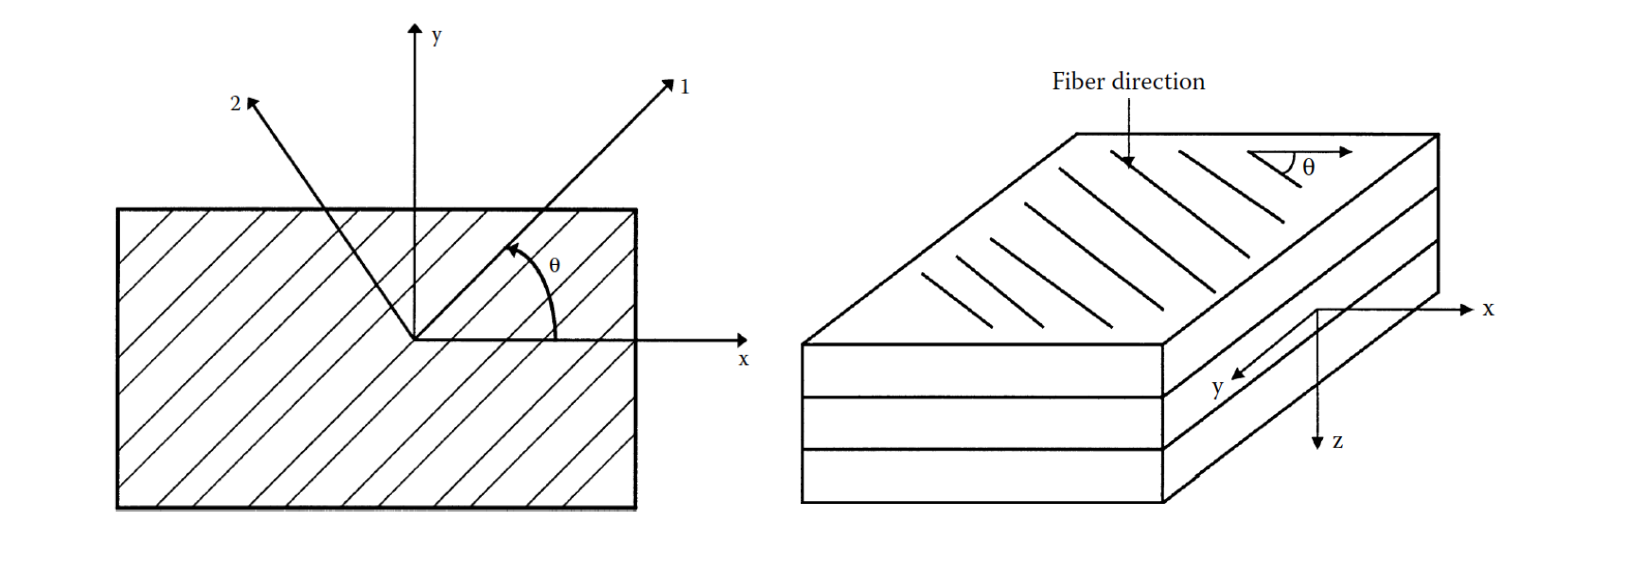
\includegraphics[width=1\linewidth]{Figures/chapter5/fig/lamina_local_global_axes.png}
	\caption{The left diagram shows the local and global axis of an angle lamina, which is from a laminate as shown in the right diagram.}
	\label{fig:lamina_local_and_global}
\end{figure}

Special cases of laminates, i.e., symmetric laminates, cross-ply laminates, are
important in the design of laminated structures. A laminate is called an angle
ply laminate if it has plies of the same material and thickness and only
oriented at $+\theta$ and $-\theta$ directions. A model of an angle ply
laminate is as shown in Fig. \ref{fig:angle-ply}.  

\begin{figure}[b]
\centering
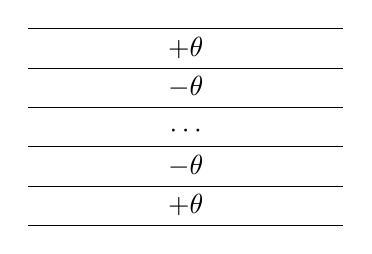
\begin{tikzpicture}
	\draw (0,0) -- (4,0);
	\draw (0,-0.5) -- (4,-0.5) node[midway, above] {$\mathit{+}\theta$};
	\draw (0,-1) -- (4,-1) node[midway, above] {$\mathit{-}\theta$} ;
	\draw (0,-1.5) -- (4,-1.5) node[midway, above] {$\cdots$};
	\draw (0,-2) -- (4,-2) node[midway, above] {$\mathit{-}\theta$};
	\draw (0,-2.5) -- (4,-2.5) node[midway, above] {$\mathit{+}\theta$};
\end{tikzpicture}
\caption{Model for angle ply laminate}
\label{fig:angle-ply}
\end{figure}


\subsubsection{Stress and Strain in a Lamina}
For a single lamina under in-plane loading whose thickness is relatively small,
suppose the upper and lower surfaces of the lamina are free from external
loading. According to Hooke's law, the three-dimensional stress-strain
equations can be reduced to two-dimensional stress-strain equations in the
composite material. The stress-strain relation in local axis 1-2 is
\begin{equation}
	\left[
		\begin{array}{l}
        	\sigma _1\\
        	\sigma _2\\
        	\tau_{12}
    	\end{array}
	\right]
    =
	\left[
		\begin{array}{ccc}
        	Q_{11} & Q_{12} & 0\\
        	Q_{12} & Q_{22} & 0\\
        	0      & 0     & Q_{66}
    	\end{array}
	\right]
	\left[
		\begin{array}{l}
        	\varepsilon_1\\
        	\varepsilon_2\\
			\gamma_{12}
		\end{array} 
	\right]
\end{equation}
where $Q_{ij} $ are the stiffnesses of the lamina. And they are related to
engineering elastic constants as follows:
\begin{equation}
	\begin{array}{l}
		Q_{11}=\frac{E_1}{1-v_{12}v_{21}} \textstyle{,} \\
    	Q_{22}=\frac{E_2}{1-v_{12}v_{21}} \textstyle{,}\\
    	Q_{66}=G_{12} \textstyle{,}\\
    	Q_{12}=\frac{v_{21}E_2}{1-v_{12}v_{21}} \textstyle{,}
    \end{array}
\end{equation}
where $E_1, E_2, v_{12}, G_{12} $ are four independent engineering elastic
constants, which are defined as follows: $E_1 $ is the longitudinal Young's
modulus, $E_2 $ is the transverse Young's modulus, $v_{12} $ is the major
Poisson's ratio, and $G_{12} $ is the in-plane shear modulus.

Stress strain relation in the global x-y axis is
\begin{equation}
	\label{equ:stress-strain}
	\left[\begin{array}{l}
			\sigma _{x} \\ 
			\sigma _{y} \\
			\tau_{xy}
			\end{array}
	\right]=
	\left[\begin{array}{lll}
			\bar{Q}_{11} & \bar{Q}_{12} & \bar{Q}_{16}\\ 
			\bar{Q}_{12} & \bar{Q}_{22} & \bar{Q}_{26} \\
			\bar{Q}_{16} & \bar{Q}_{26} &\bar{Q}_{66}
		\end{array}
	 \right]
	 \left[\begin{array}{l}
			 \varepsilon_{x} \\ 
	 		 \varepsilon_{y} \\ 
	 		 \gamma_{x y}
	 		\end{array}
	\right] 
\end{equation}
where
\begin{equation}
	\begin{array}{l}
		\resizebox{.35\textwidth}{!}{$\bar{Q}_{11}=Q_{11} cos^{4}\theta+Q_{22} sin^{4}\theta+2\left(Q_{12}+2
		Q_{66}\right) sin^{2}\theta cos^{2}\theta$}\textstyle{,} \\
		\resizebox{.35\textwidth}{!}{$\bar{Q}_{12}=\left(Q_{11}+Q_{22}-4 Q_{66}\right) sin^{2}\theta
			cos^{2}\theta+Q_{12}\left(cos^{4}\theta+sin^{2}\theta \right)$} \textstyle{,}\\
		\resizebox{.35\textwidth}{!}{$\bar{Q}_{22}=Q_{11} sin^{4}\theta+Q_{22} cos^{4}\theta+2\left(Q_{12}+2
				Q_{66}\right) sin^{2}\theta cos^{2}\theta$}\textstyle{,} \\
		\resizebox{.40\textwidth}{!}{$\bar{Q}_{16}=\left(Q_{11}-Q_{12}-2
			Q_{66}\right) cos^{3}\theta
			sin\theta-\left(Q_{22}-Q_{12}-2Q_{66}\right) sin^{3}\theta cos\theta$} \textstyle{,}\\ 
		\resizebox{.40\textwidth}{!}{$\bar{Q}_{26}=\left(Q_{11}-Q_{12}-2
			Q_{66}\right) cos\theta sin^{3}\theta-\left(Q_{22}-Q_{12}-2
			Q_{66}\right)cos^{3}\theta sin\theta$} \textstyle{,}\\ 
		\resizebox{.40\textwidth}{!}	{$\bar{Q}_{66}=\left(Q_{11}+Q_{22}-2 Q_{12}-2 Q_{66}\right)
			sin\theta^{2}cos\theta^{2}+Q_{66}\left(sin\theta^{4}+cos\theta^{4}\right)$}\textstyle{.}\\
	\end{array}
\end{equation}

\subsubsection{Stress and Strain in a Laminate}
For forces and moment resultants acting on laminates, such as in plate and shell
structures, the relationship between applied forces and moment and displacement
can be given by

\begin{equation} \label{eq:force_and_moments}
	\begin{array}{ll}
	\begin{bmatrix}
		N_x \\
		N_y \\
		N_{xy}
	\end{bmatrix}
	&=
	\begin{bmatrix}
		A_{11} & A_{12} & A_{16} \\
		A_{12} & A_{22} & A_{26} \\
		A_{16} & A_{26} & A_{66} 
	\end{bmatrix}
    \begin{bmatrix}
		\varepsilon_x^0 \\
        \varepsilon_y^0 \\
		\gamma_{xy}^0
    \end{bmatrix}   \\
	&+               
	\begin{bmatrix}
		B_{11} & B_{12} & B_{16} \\
		B_{11} & B_{12} & B_{16} \\
		B_{16} & B_{26} & B_{66} 
	\end{bmatrix}
	\begin{bmatrix}
		k_x \\
		k_y \\
		k_{xy} 
	\end{bmatrix}  \textstyle{,}
	\end{array}
\end{equation}
where $N_x,N_y $ refers to the normal force per unit length;
$N_{xy}$ means shear force per unit length;
$\varepsilon^{0}$ and $k_{xy}$ denotes  mid plane strains and curvature of a laminate in x-y coordinates
The mid-plane strain and curvature is given by
\begin{equation}
    \begin{split}
	&A_{ij}=\sum_{k=1}^{n}(\overline{Q_{ij}})_k(h_k-h_{k-1})  i=1,2,6, j=1,2,6 \textstyle{,}\\
    &B_{ij}=\frac{1}{2}\sum_{k=1}^{n}(\overline{Q_{ij}})_k(h_k^2 - h_{k-1}^2)  i=1,2,6, j=1,2,6\textstyle{,}\\
    &D_{ij}=\frac{1}{3}\sum_{k=1}^{n}(\overline{Q_{ij}})_k(h_k^3 - h_{k-1}^3) i=1,2,6, j=1,2,6\textstyle{.}\\
    \end{split}
\end{equation}

The [A], [B], and [D] matrices are called the extensional, coupling, and bending stiffness matrices,
respectively. The extensional stiffness matrix $[A]$ relates the resultant in-plane forces to the
in-plain strains, and the bending stiffness matrix $[D]$ couples the resultant bending moments to
the plane curvatures.  The coupling stiffness matrix $[B]$ relates the force and moment terms to the
midplain strains and midplane curvatures.

\subsection{Failure criteria for a lamina}

Failure criteria for composite materials are more difficult to predict due to
structural and material complexity in comparison to isotropic materials. The
failure process of composite materials can be regarded from microscopic and
macroscopic points of view. Most popular criteria about the failure of an angle
lamina are in terms of macroscopic failure criteria, which are based on the
tensile, compressive, and shear strengths. According to the failure surfaces,
these criteria
\cite{massard1984computer,reddy1987first,fang1993design,soeiro1994multilevel,pelletier2006multi,jadhav2007parametric,omkar2008artificial,choudhury2019failure},
can be classified into two classes: one is called independent failure mode
criteria which includes the maximum stress failure
theory\cite{watkins1987multicriteria}, maximum strain failure theory because
their failure envelop are rectangle; another is called quadratic polynomial
which includes Tsai-Wu\cite{martin1987optimum,soares1995discrete}, Chamis,
Hoffman and Hill criteria because their failure surfaces are of ellipsoidal
shape. In the present study, the two most reliable failure criteria are taken,
Maximum stress and Tsai-wu.  Both of these two failure criteria are based on
the stresses in the local axis instead of principal normal stresses and maximum
shear stresses, and four normal strength parameters and one shear stress for a
unidirectional lamina are involved. The five strength parameters are

$(\sigma _1^{T})_{ult}= $ ultimate longitudinal tensile strength(in direction 1),

$(\sigma _1^{C})_{ult}= $ ultimate longitudinal compressive strength,

$(\sigma _2^{T})_{ult}= $ ultimate transverse tensile strength,

$(\sigma _2^{C})_{ult}= $ ultimate transverse compressive strength, and

$(\tau_{12})_{ult}= $ and ultimate in-plane shear strength.

\begin{figure}[ht]
\centering
\begin{tikzpicture}
	\begin{scope}
		%\draw[style=help lines] (-3,-3) grid (3,3);
		\draw (0,0) rectangle (2,3);
		\draw[->] (1.3,1.2) -- (2.6,1.2);
		\draw[->] (1.3,1.2) -- (1.3,3.4);
		\node at (2.2,1) {$X_T$};
		\node at (1.5, 3.2) {$Y_T$};
		\node at (-0.2, 0.9) {$X_C$};
		\node at (1.8, -0.2) {$Y_C$};
	\end{scope}
	\begin{scope}[xshift=6cm,yshift=1.15cm]
		%\draw[style=help lines] (-3,-3) grid (3,3);
		\draw[rotate=30] (0,0) ellipse (2cm and 1cm);
		\draw[->] (0.2,0) -- (0.2,2.2);
		\draw[->] (0.2,0) -- (1.9,0);
		\node at (1.6,-0.2) {$X_T$};
		\node at (0.3, 1.3) {$Y_T$};
		\node at (-1.6, 0) {$X_C$};
		\node at (-0.5, -1.5) {$Y_C$};
	\end{scope}
\end{tikzpicture}
\caption{Schematic failure surfaces for maximum stress and quadratic failure
criteria}
\label{fig:failure_surface}
\end{figure}

\subsubsection{Maximum stress(MS) failure criterion}
Maximum stress failure theory consists of maximum normal stress theory proposed
by Rankine and maximum shearing stress theory proposed by Tresca. The stress
applied on a lamina can be resolved into the normal and shear stress in the
local axis. If any of the normal or shear stresses in the local axis of a
lamina is equal or exceeds the corresponding ultimate strengths of the
unidirectional lamina, the lamina is considered to be failed. That is,

\begin{equation}
	\begin{array}{lll}
		\sigma_1 \geq (\sigma _1^{T})_{ult} & \textstyle{ or } &  \sigma_1 \leq -(\sigma _1^{C})_{ult} \textstyle{,} \\
		\sigma_2 \geq (\sigma _2^{T})_{ult} & \textstyle{ or } &   \sigma_2 \leq -(\sigma _2^{C})_{ult} \textstyle{,} \\
		\tau_{12} \geq (\tau_{12})_{ult}    & \textstyle{ or } &     \tau_{12} \leq -(\tau_{12})_{ult}  \textstyle{,}
\end{array}
\end{equation}

where $\sigma_1$ and $\sigma_2$ are the normal stresses in the local axis 1 and 2;
$\tau_{12}$ is the shear stress in the symmetry plane 1-2.

\subsubsection{Tsai-wu failure criterion}
The TW criterion is one of the most reliable static failure criteria derived from the von
Mises yield criterion.  
A lamina is considered to fail
if \begin{equation} \label{eq:tsai_wu}
\begin{split}
	H_1 \sigma_1  & + H_2 \sigma_2 + H_6 \tau_{12} + H_{11}\sigma_1^2 + H_{22} \sigma_2^2 \\
				  & + H_{66}  \tau_{12}^2 + 2H_{12}\sigma_1\sigma_2 < 1
\end{split}
\end{equation}

is violated, where

\begin{equation}
	\begin{split}
		H_{1}&=\frac{1}{\left(\sigma_{1}^{T}\right)_{u l t}}-\frac{1}{\left(\sigma_{1}^{C}\right)_{u l t}}\textstyle{,} \\
		H_{11}&=\frac{1}{\left(\sigma_{1}^{T}\right)_{u l t}\left(\sigma_{1}^{C}\right)_{u l t}} \textstyle{,}\\
		H_{2}&=\frac{1}{\left(\sigma_{2}^{T}\right)_{u l t}}-\frac{1}{\left(\sigma_{2}^{C}\right)_{u l t}} \textstyle{,}\\
		H_{22}&=\frac{1}{\left(\sigma_{2}^{T}\right)_{u l t}\left(\sigma_{2}^{C}\right)_{u l t}} \textstyle{,}\\
		H_{66}&=\frac{1}{\left(\tau_{12}\right)_{u l t}^{2}} \textstyle{,}\\
		H_{12}&=-\frac{1}{2} \sqrt{\frac{1}{\left(\sigma_{1}^{T}\right)_{u l
		t}\left(\sigma_{1}^{C}\right)_{u l t}\left(\sigma_{2}^{T}\right)_{u l
		t}\left(\sigma_{2}^{C}\right)_{u l t}}}\textstyle{.}
	\end{split}
\end{equation}

$H_i$ is the strength tensors of the second-order; $H_{ij}$ is the strength
tensors of the fourth-order. $\sigma_1$ is the applied normal stress in 
direction 1; $\sigma_2$ is the applied normal stress in direction 2; 
$\tau_{12}$ is the applied in-plane shear stress.




\subsubsection{Strength ratio}
The safety factor, or yield stress, is how much extra load beyond is intended a
composite laminate will take. The strength ratio is defined as 

\begin{equation}
	\label{eq:sr}S R=\frac{\text {Maximum Load Which Can Be Applied}}{\text {Load Applied}}
\end{equation}.
